\section{Diskussion}
\label{sec:Diskussion}
\sisetup{range-phrase = { bis }, locale = DE}

\begin{table}
  \centering
  \caption{Elastizitätsmodul $E$ der beiden Stäbe, bestimmt mit den drei Messverfahren, im Vergleich zu den Literaturwerten \cite{Aluminium}.}
  \label{tab:E_vergleich}
  \begin{tabular}{l S[table-format=3.1(2)] S[table-format=3.1(2)]}
    \toprule
    {Methode} & {Stab 1 (Al) $E/\unit{\giga\pascal}$} & {Stab 2 (Cu) $E/\unit{\giga\pascal}$} \\
    \midrule
    Einseitige Einspannung       & 59.6(14)  & 154.7(31) \\
    Zweiseitige Auflage (links)  & 156.6(53) & {--} \\
    Zweiseitige Auflage (rechts) & 92.3(25)  & {--} \\
    Schallgeschwindigkeit        & 63.0(23)  & 146.8(49) \\
    \midrule
    Literaturwert                & {70}      & {\numrange{110}{130}} \\
    \bottomrule
  \end{tabular}
\end{table}
Tabelle~\ref{tab:E_vergleich} stellt die bestimmten Elastizitätsmodule den
Literaturwerten gegenüber. Die relative Abweichung wird dabei als
$\left|E_\text{exp} - E_\text{lit}\right| / E_\text{lit}$ angegeben.

Für Stab 1 liefern die einseitige Einspannung ($E = \SI{59.6(14)}{\giga\pascal}$)
und die Schallgeschwindigkeitsmessung ($E = \SI{63.0(23)}{\giga\pascal}$) zueinander
passende Werte, die etwas unterhalb des Literaturwertes für Aluminium von
\SI{70}{\giga\pascal} liegen. Die relativen Abweichungen betragen \SI{14.9}{\percent}
bzw. \SI{10.0}{\percent}. Beide Werte sind damit für eine Aluminium-Legierung
plausibel, da das Elastizitätsmodul je nach Legierung schwankt.
Die Ergebnisse der zweiseitigen Auflage
($E_\text{links} = \SI{156.6(53)}{\giga\pascal}$,
$E_\text{rechts} = \SI{92.3(25)}{\giga\pascal}$) weichen mit \SI{124}{\percent} bzw.
\SI{32}{\percent} stark vom Literaturwert und deutlich voneinander ab. Sie
erlauben daher keine klare Aussage über das Elastizitätsmodul des Stabes.
Mögliche Ursachen werden in Abschnitt~\ref{sec:Fehlerquellen} diskutiert. %%Fehlerquellen ergänzen

Für Stab 2 liegen beide Messwerte oberhalb des Literaturbereichs für Kupfer von
\SIrange{110}{130}{\giga\pascal}. Die Schallgeschwindigkeitsmessung
($E = \SI{146.8(49)}{\giga\pascal}$) weicht um \SI{22}{\percent} vom Mittelwert
\SI{120}{\giga\pascal} ab, die einseitige Einspannung
($E = \SI{154.7(31)}{\giga\pascal}$) um \SI{29}{\percent}. Auch gegenüber der
Obergrenze von \SI{130}{\giga\pascal} bleiben Abweichungen von \SI{13}{\percent}
bzw. \SI{19}{\percent}. Die beiden Verfahren stimmen untereinander besser
überein als mit der Literatur, was auf einen systematischen Fehler oder
eine abweichende Zusammensetzung des Stabes hindeutet.

\subsection{Fehlerquellen}
\label{sec:Fehlerquellen}
Bei der experimentellen Bestimmung der Biegung können verschiedene Einflüsse zu Abweichungen zwischen den theoretisch berechneten und den gemessenen Werten führen. \\
Eine Fehlerquelle sind Ungenauigkeiten bei der Messung der Stäbe. Da bereits kleine Abweichungen bei der Dicke, Breite oder dem Durchmesser einen großen Einfluss auf das Flächenträgheitsmoment haben, können Messfehler das Ergebnis deutlich verfälschen. Auch Unterschiede im Querschnitt entlang des Stabes können eine Rolle spielen. \\
\subsubsection{Fehlerquellen bei der Durchbiegung eines einseitig und beidseitig eingespannten homogenen Stabes}
Eine mögliche Fehlerquelle ist die elastische Nachwirkung. Dabei verformt sich ein Material nicht sofort vollständig, sondern erst mit einer gewissen Verzögerung. Die Messung über die Schallgeschwindigkeit ist davon nicht betroffen.\\
Weitere Fehler können durch den Versuchsaufbau entstehen. Während der Messung konnten wir feststellen, dass bereits leichte Bewegungen oder Erschütterungen der Vorrichtung zu Veränderungen der angezeigten Messwerte führten.\\
Auch die Einspannung und die Auflagepunkte können eine Fehlerquelle sein. In der Theorie wird angenommen, dass die Einspannung festsitzt und die Auflagepunkte genau positioniert sind. In der Praxis können diese jedoch leicht nachgeben, verrutschen oder nicht ganz waagerecht sein. Die Reibung wurde dabei auch komplett vernachlässigt.\\
Bei der beidseitigen Auflage waren die beiden Enden unterschiedlich befestigt. Während auf ein Ende von oben Druck ausgeübt wurde, lag das andere Ende lediglich in einer Vorrichtung und wurde durch eine Schraube gegen ein Verschieben in Längsrichtung gesichert (siehe Abbildung \ref{fig:BiegungA22}). Diese Befestigung wirkte jedoch nicht besonders stabil. Dies könnte eine mögliche Ursache für die deutlichen Unterschiede zwischen den gemessenen und den theoretisch berechneten Werten darstellt.\\
Außerdem ist es bei der beidseitigen Einspannung wichtig, dass alle Abstände möglichst genau eingehalten werden. Besonders die Positionen der beiden Messuhren sowie die Platzierung des Gewichts genau in der Mitte sind dabei entscheidend. Bereits kleine Abweichungen bei der Ausrichtung oder Positionierung können das Messergebnis beeinflussen und zu deutlichen Unterschieden zwischen den gemessenen und den theoretisch berechneten Werten führen. Dadurch ist diese Versuchsanordnung besonders fehleranfällig.
\begin{figure}[H]
    \centering
    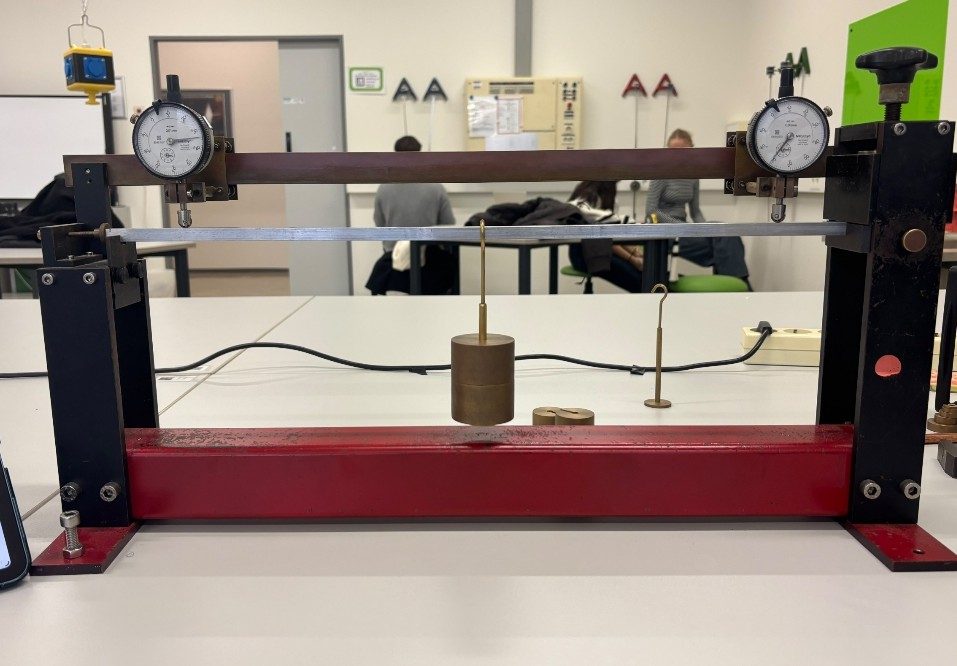
\includegraphics[width=0.8\textwidth]{BiegungA22.jpg}
    \caption{unsere benutze Apparatur für die Messungen}
    \label{fig:BiegungA22}
\end{figure}
\subsubsection{Fehlerquellen bei der Bestimmung durch Schallgeschwindigkeit}
Auch bei der Schallmessung können verschiedene Fehlerquellen auftreten. Eine davon ist die Ankopplung des Tonabnehmers. Wenn dieser nicht richtig am Stab sitzt oder die Schallimpulse unterschiedlich stark aufnimmt, kann es zu Ungenauigkeiten bei der Zeitmessung kommen.\\
Zusätzlich ist die Art der Stoßanregung entscheidend. Die Stahlkugel sollte möglichst gerade und mittig auf den Stab treffen, damit sich die Schallwelle gleichmäßig ausbreitet und keine zusätzlichen Schwingungen entstehen.\\
Eine weitere Fehlerquelle ist der Energieverlust des Schallimpulses. Bei jeder Reflexion an den Stabenden verliert dieser etwas Energie und wird dadurch schwächer. Bei vielen Reflexionen kann das Signal schließlich so schwach werden, dass es vom Messgerät nichtmehr eindeutig erkannt wird. Dadurch können Fehler bei der Zeitmessung entstehen.\\
\subsection{Fazit}
Beim ersten Stab aus einer Aluminiumlegierung lieferten sowohl die einseitige Einspannung als auch die Schallgeschwindigkeitsmessung plausible Ergebnisse, die gut mit dem Literaturwert übereinstimmten. Die zweiseitige Auflagerung zeigte hingegen deutliche Abweichungen. Dies lässt sich vermutlich auf die instabile Lagerung und Ungenauigkeiten bei der Positionierung zurückführen. Die Ergebnisse dieser Messung sind daher nur eingeschränkt aussagekräftig. Eine Wiederholung des Versuchs mit einem stabileren und genaueren Versuchsaufbau wäre sinnvoll, um zuverlässigere Werte zu erhalten.\\
Für den zweiten Stab aus Kupfer, stimmen die Werte aus einseitiger Einspannung und Schallmessung gut untereinander überein, liegen jedoch systematisch oberhalb des Literaturbereichs für reines Kupfer, was auf eine abweichende Legierungszusammensetzung oder geometrische Messunsicherheiten hindeutet. \\
Insgesamt hat sich die Bestimmung über die Schallgeschwindigkeit als das präziseste und am wenigsten störanfällige Verfahren erwiesen, da hierbei Effekte wie elastische Nachwirkung und Lagerungsfehler entfallen.